\documentclass[a4paper,11pt]{article}
\usepackage[utf8]{inputenc}
\usepackage[ngerman]{babel}
\usepackage{geometry}
\usepackage{graphicx}
\usepackage{amsmath}
\usepackage{hyperref}
\usepackage{enumitem}

\geometry{a4paper, top=2cm, bottom=2cm, left=2cm, right=2cm}	

\usepackage{xcolor}
\definecolor{ohm_red}{RGB}{192,0,0}


\usepackage{fancyhdr}


\usepackage{titling}
\pretitle{\begin{flushleft}\LARGE}
\posttitle{\end{flushleft}}
\preauthor{\begin{flushleft}\large}
\postauthor{\end{flushleft}}

\setlength{\parindent}{0pt}



\pretitle{\begin{flushleft}\huge\textbf{\textcolor{ohm_red}}}
\posttitle{\end{flushleft}}

\pretitle{\begin{flushleft}\huge\textbf{\textcolor{ohm_red}}\rule{\linewidth}{0.4mm}\\}
\posttitle{\\\rule{\linewidth}{0.4mm}\end{flushleft}}
\title{\textcolor{ohm_red}{3D-Kartierung und Perzeption in der Such- und Erkundungsrobotik}}

\date{}


\usepackage{enumitem}
\setlist{nosep}

\pagestyle{fancy}
\renewcommand{\headrulewidth}{0pt}
\fancyhead[L]{
\includegraphics[height=2.0cm]{img/logo_autonohm.png}}
\fancyhead[R]{veröffentlicht am \today}


\usepackage{sidecap}

\sidecaptionvpos{figure}{c}


\begin{document}

\maketitle
\thispagestyle{fancy}

\vspace*{-3cm}
\begin{figure}[h!]
    \centering
    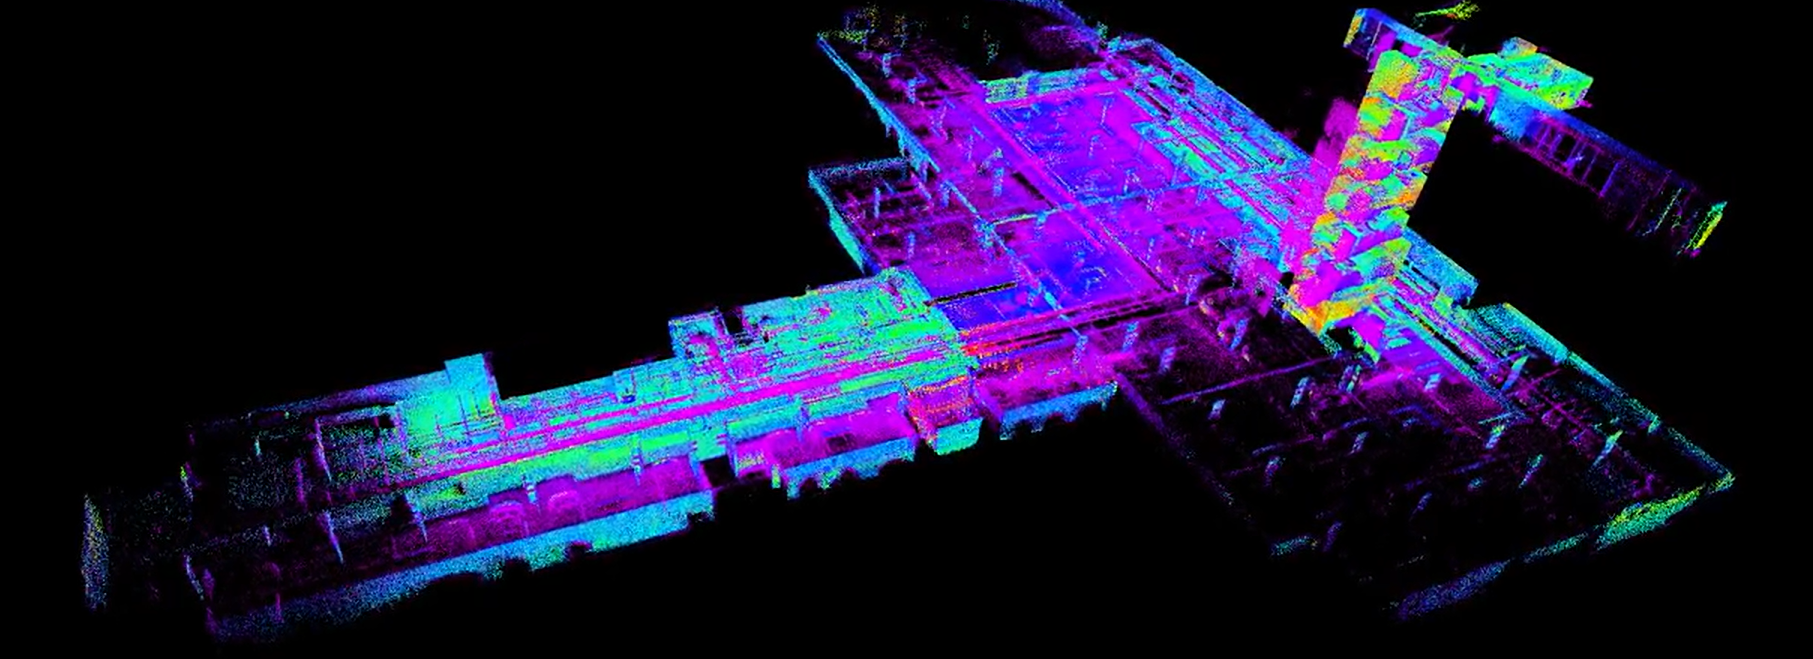
\includegraphics[height=4cm]{img/livox_map.png}
    % \caption{Example Image}
    % \label{fig:example}
\end{figure}

Das Erstellen von präzisen 3D-Karten ist ein wichtiger Bestandteil in der Such- und Erkundungsrobotik. Die Karten dienen als Grundlage für die autonome Navigation und die Erkennung von Objekten. Im Labor für mobile Robotik existiert ein \href{https://www.livoxtech.com/de/mid-360}{Livox mid 360 LiDAR-Sensor}, der zur Erstellung von 3D-Karten eingesetzt werden kann. In dieser Arbeit soll ein ROS-System aufgebaut werden, das die 3D-Kartierung und Perzeption in der Such- und Erkundungsrobotik ermöglicht, basierend auf dem Livox LiDAR-Sensor und Bilddaten. So sollen wichtige Gegenstände in der Umgebung erkannt, lokalisiert und in eine Umgebungskarte eingetragen werden.
Eine mögliche Implementierung zeigt das Video \href{https://www.youtube.com/watch?v=adALW9jCwtc}{hier}.
Für die Implementierung kann auf bestehende open-source Softwarepakete zurückgegriffen werden. 

\section*{Arbeitspakete}
\begin{itemize}[leftmargin=0.5cm]
    \item Recherche von Softwarepaketen für die 3D-Kartierung
    \item Implementierung einer 3D-Kartierung mit dem Livox LiDAR-Sensor
    \item Implementierung einer Objekterkennung und Lokalisierung
    \item Test und Evaluation 
\end{itemize}

\section*{Voraussetzungen}
\begin{itemize}[leftmargin=0.5cm]
    \item Grundkenntnisse in ROS 
    \item Grundkenntnisse in einer höheren Programmiersprache (z.B. Python, C++)
    \item Grundkenntnisse in der Robotik
\end{itemize}

\vspace{0.5cm}
Das Thema kann nach Abstimmung als Bachelor- oder Masterarbeit bearbeitet werden, sowie als Projektarbeit. 


\vfill
\textcolor{ohm_red}{\rule{\linewidth}{0.4mm}}
\textbf{\textcolor{ohm_red}{Labor für mobile Robotik}} \\
\begin{tabular}{@{}ll}
\textbf{Betreuer:} & Prof. Dr. Christian Pfitzner \\
\textbf{E-Mail:}   & \href{mailto:christian.pfitzner@th-nuernberg.de}{christian.pfitzner@th-nuernberg.de} \\
\end{tabular}

\end{document}